
\documentclass{article}
\usepackage[utf8]{inputenc}
\usepackage{pgf}
\usepackage{tikz}
\usetikzlibrary{arrows,automata,positioning}
\usepackage{polski}
\usepackage{amsmath}
\usepackage{amssymb}
\usepackage{amsfonts}
\begin{document}

\begin{figure}[ht]
\centering
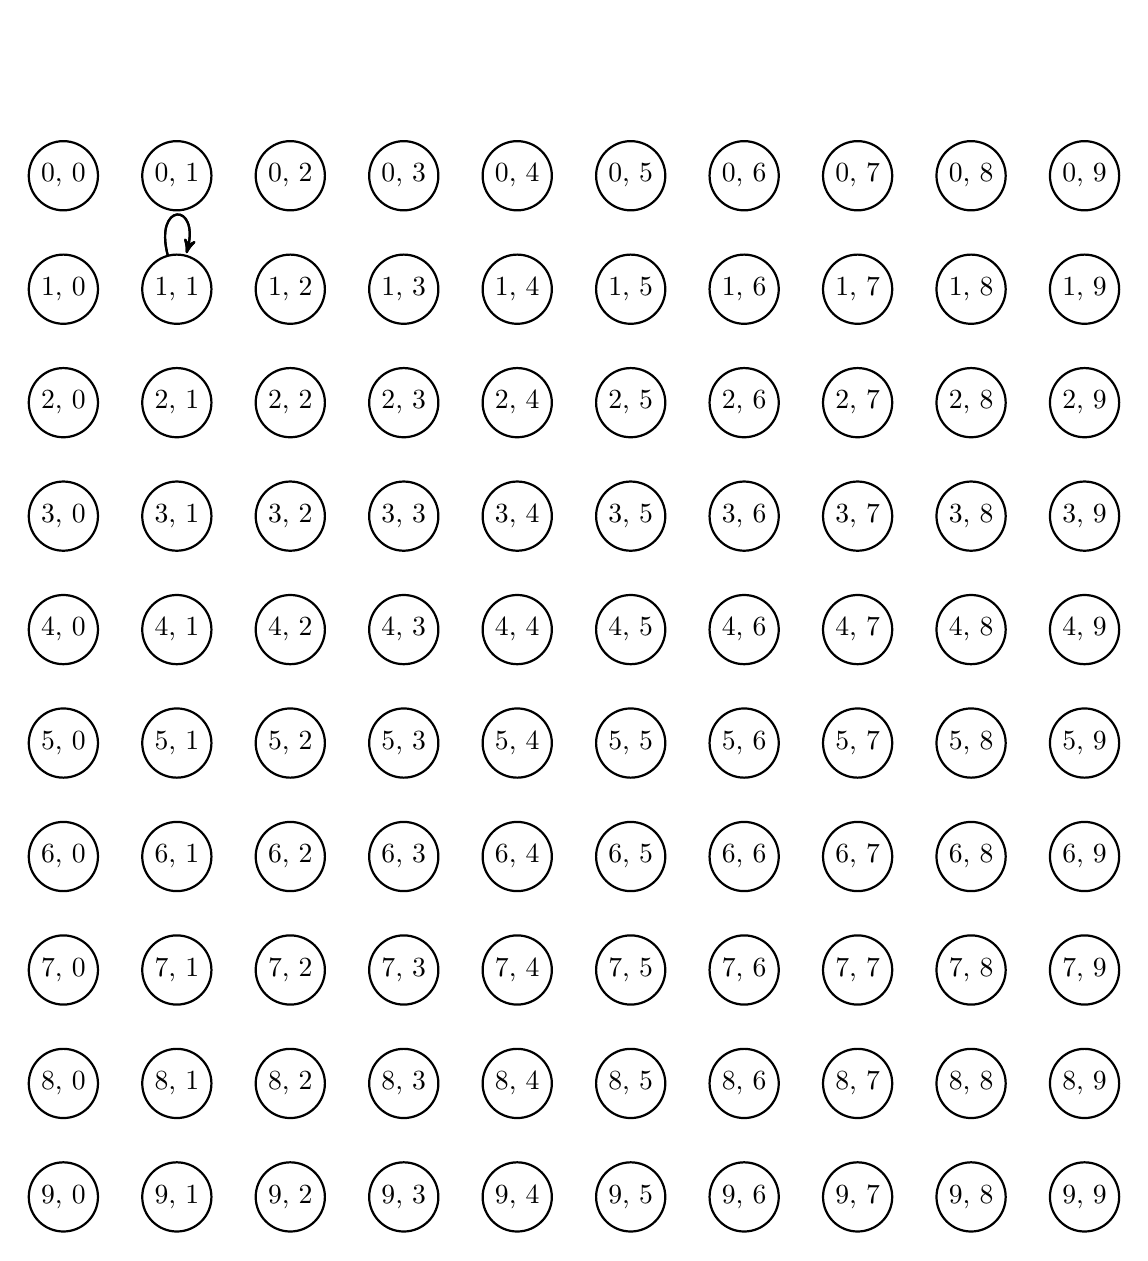
\begin{tikzpicture}[y=0.80pt, x=0.80pt, yscale=1, xscale=1, inner sep=0pt, outer sep=0pt, 
->,>=stealth',shorten >=1pt,auto, thick, trans/.style={thick,->,>=stealth}]
  \node[state, draw=none] (X)                    {};
\node[state](I00)[below = 20 of X] {0, 0};
\node[state](I01)[right = 20 of I00] {0, 1};
\node[state](I02)[right = 20 of I01] {0, 2};
\node[state](I03)[right = 20 of I02] {0, 3};
\node[state](I04)[right = 20 of I03] {0, 4};
\node[state](I05)[right = 20 of I04] {0, 5};
\node[state](I06)[right = 20 of I05] {0, 6};
\node[state](I07)[right = 20 of I06] {0, 7};
\node[state](I08)[right = 20 of I07] {0, 8};
\node[state](I09)[right = 20 of I08] {0, 9};
\node[state](I10)[below = 20 of I00] {1, 0};
\node[state](I11)[right = 20 of I10] {1, 1};
\node[state](I12)[right = 20 of I11] {1, 2};
\node[state](I13)[right = 20 of I12] {1, 3};
\node[state](I14)[right = 20 of I13] {1, 4};
\node[state](I15)[right = 20 of I14] {1, 5};
\node[state](I16)[right = 20 of I15] {1, 6};
\node[state](I17)[right = 20 of I16] {1, 7};
\node[state](I18)[right = 20 of I17] {1, 8};
\node[state](I19)[right = 20 of I18] {1, 9};
\node[state](I20)[below = 20 of I10] {2, 0};
\node[state](I21)[right = 20 of I20] {2, 1};
\node[state](I22)[right = 20 of I21] {2, 2};
\node[state](I23)[right = 20 of I22] {2, 3};
\node[state](I24)[right = 20 of I23] {2, 4};
\node[state](I25)[right = 20 of I24] {2, 5};
\node[state](I26)[right = 20 of I25] {2, 6};
\node[state](I27)[right = 20 of I26] {2, 7};
\node[state](I28)[right = 20 of I27] {2, 8};
\node[state](I29)[right = 20 of I28] {2, 9};
\node[state](I30)[below = 20 of I20] {3, 0};
\node[state](I31)[right = 20 of I30] {3, 1};
\node[state](I32)[right = 20 of I31] {3, 2};
\node[state](I33)[right = 20 of I32] {3, 3};
\node[state](I34)[right = 20 of I33] {3, 4};
\node[state](I35)[right = 20 of I34] {3, 5};
\node[state](I36)[right = 20 of I35] {3, 6};
\node[state](I37)[right = 20 of I36] {3, 7};
\node[state](I38)[right = 20 of I37] {3, 8};
\node[state](I39)[right = 20 of I38] {3, 9};
\node[state](I40)[below = 20 of I30] {4, 0};
\node[state](I41)[right = 20 of I40] {4, 1};
\node[state](I42)[right = 20 of I41] {4, 2};
\node[state](I43)[right = 20 of I42] {4, 3};
\node[state](I44)[right = 20 of I43] {4, 4};
\node[state](I45)[right = 20 of I44] {4, 5};
\node[state](I46)[right = 20 of I45] {4, 6};
\node[state](I47)[right = 20 of I46] {4, 7};
\node[state](I48)[right = 20 of I47] {4, 8};
\node[state](I49)[right = 20 of I48] {4, 9};
\node[state](I50)[below = 20 of I40] {5, 0};
\node[state](I51)[right = 20 of I50] {5, 1};
\node[state](I52)[right = 20 of I51] {5, 2};
\node[state](I53)[right = 20 of I52] {5, 3};
\node[state](I54)[right = 20 of I53] {5, 4};
\node[state](I55)[right = 20 of I54] {5, 5};
\node[state](I56)[right = 20 of I55] {5, 6};
\node[state](I57)[right = 20 of I56] {5, 7};
\node[state](I58)[right = 20 of I57] {5, 8};
\node[state](I59)[right = 20 of I58] {5, 9};
\node[state](I60)[below = 20 of I50] {6, 0};
\node[state](I61)[right = 20 of I60] {6, 1};
\node[state](I62)[right = 20 of I61] {6, 2};
\node[state](I63)[right = 20 of I62] {6, 3};
\node[state](I64)[right = 20 of I63] {6, 4};
\node[state](I65)[right = 20 of I64] {6, 5};
\node[state](I66)[right = 20 of I65] {6, 6};
\node[state](I67)[right = 20 of I66] {6, 7};
\node[state](I68)[right = 20 of I67] {6, 8};
\node[state](I69)[right = 20 of I68] {6, 9};
\node[state](I70)[below = 20 of I60] {7, 0};
\node[state](I71)[right = 20 of I70] {7, 1};
\node[state](I72)[right = 20 of I71] {7, 2};
\node[state](I73)[right = 20 of I72] {7, 3};
\node[state](I74)[right = 20 of I73] {7, 4};
\node[state](I75)[right = 20 of I74] {7, 5};
\node[state](I76)[right = 20 of I75] {7, 6};
\node[state](I77)[right = 20 of I76] {7, 7};
\node[state](I78)[right = 20 of I77] {7, 8};
\node[state](I79)[right = 20 of I78] {7, 9};
\node[state](I80)[below = 20 of I70] {8, 0};
\node[state](I81)[right = 20 of I80] {8, 1};
\node[state](I82)[right = 20 of I81] {8, 2};
\node[state](I83)[right = 20 of I82] {8, 3};
\node[state](I84)[right = 20 of I83] {8, 4};
\node[state](I85)[right = 20 of I84] {8, 5};
\node[state](I86)[right = 20 of I85] {8, 6};
\node[state](I87)[right = 20 of I86] {8, 7};
\node[state](I88)[right = 20 of I87] {8, 8};
\node[state](I89)[right = 20 of I88] {8, 9};
\node[state](I90)[below = 20 of I80] {9, 0};
\node[state](I91)[right = 20 of I90] {9, 1};
\node[state](I92)[right = 20 of I91] {9, 2};
\node[state](I93)[right = 20 of I92] {9, 3};
\node[state](I94)[right = 20 of I93] {9, 4};
\node[state](I95)[right = 20 of I94] {9, 5};
\node[state](I96)[right = 20 of I95] {9, 6};
\node[state](I97)[right = 20 of I96] {9, 7};
\node[state](I98)[right = 20 of I97] {9, 8};
\node[state](I99)[right = 20 of I98] {9, 9};
\path 
(I11) edge [loop above] node {} (I11)
(I11) edge [loop above] node {} (I11)
;
\end{tikzpicture}
\label{fig:figure2}
\end{figure}


\end{document}
